\chapter{Integrated Solutions}
\label{sec:integrated_solutions}

In general, an integrative work benefits from many integrated solutions. Nevertheless, it should be viable in the scope of the work and robust. Essentially, there is a tradeoff
between integrating as much as possible, thereby increasing the functionality, and staying feasible and realistic. Two solutions developed in the course of the \textit{PORTAL} project that
match very well with the framework proposed in this thesis are introduced in the following sections. Section \ref{sec:battery_monitoring} is concerned with a battery monitoring
solution, and section \ref{sec:docking_solution} presents a system that enables autonomous energy supply.

\section{Battery Monitoring}
\label{sec:battery_monitoring}

One solution worth integrating is a watchdog module developed as part of the \textit{PORTAL} project that monitors the battery state and acts as a fail-safe. In principle, the charge stops are part of the plan, i.e., are
considered at planning time. Thus, there is resource planning for the missions that includes to be back at the base station before the robot runs out of battery. However, if it fails,
there should be a monitoring process at execution time that is able to react to wrong plans, i.e., the battery is depleted before expected and the robot has to return to its base.
The module essentially checks the distance from the robot's current position to the base station, the expected battery consumption to get there, and the remaining battery charge.
Generally, the base station restricts the robot's radius of motion; the robot is, as Egerstedt et al. put it, \textquote{spatially anchored}. \cite{Egerstedt:2018} In summary, the
module is running at execution time, it does not schedule the charge stops in advance, but only responds to failure cases where the robot needs to preempt the plan execution, return
to its base and recharge. This battery watchdog is the basis for the power management failure monitoring presented in section \ref{sec:sim_and_mon_power_management}. In order for the
module to provide reasonable estimates, it is critical that the robot constantly reports its current mode of operation. The battery watchdog distinguishes between \code{scanning},
\code{traversing}, \code{waiting}, \code{docking}, \code{undocking}, \code{charging}, \code{dead}, \code{contingency} and \code{catastrophe}. All these modes are set in the operation
state machine (cf. section \ref{sec:execution_monitoring_smach_architecture}) at appropriate transitions by publishing to \code{/arox/ongoing_operation}.

\vfill
\pagebreak

\section{Autonomous Energy Supply}
\label{sec:docking_solution}

A fundamental step towards long-term autonomy of a mobile robot is to ensure its power supply. Arvin et al. \cite{Arvin:2009} emphasize autonomous navigation and precise docking at
a charging station as major problems for mobile robots, since many mobile robots require human assistance to charge. They identify three critical aspects for mobile robots that can
recharge themselves: Awareness of the need to charge, locating and navigating to the charging station, and precise docking. In order for the robot to recharge, there is an inductive
charging station, which is located in a mobile container on the field site. For the \textit{PORTAL} project, the container providing the inductive charging station was modeled in URDF
and can be used in the \textit{Gazebo} simulation (cf. fig. \ref{fig:container_model}).
\begin{figure}[H]
    \centering
    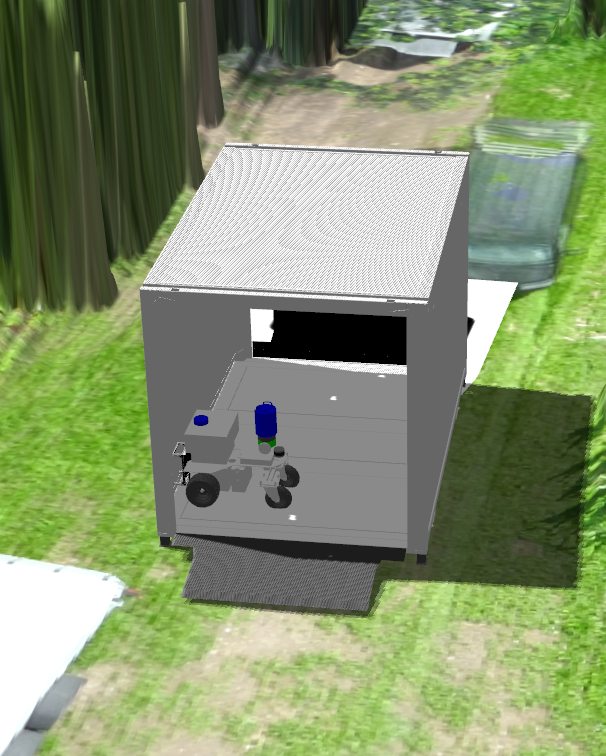
\includegraphics[width=0.35\textwidth]{img/docked.png}
    \caption{\textsc{Robot Docked to Charging Station}}
    \label{fig:container_model}
\end{figure}
\noindent
Thus, the power supply can be realized by integrating an autonomous docking / undocking solution that enables the robot to detect the container in a laser scan of its nearby
surroundings, drive into it and dock to the inductive charging station. Such a docking solution has been created as part of the \textit{PORTAL} project and is extended in this work by some
error handling mechanisms to enable meaningful monitoring. The docking solution is integrated into the framework developed in this thesis to provide the robot with autonomous
recharging capability. The component integrating the (un)docking methods into the presented framework is the operation state machine, which is responsible for the action execution
(cf. section \ref{sec:execution_monitoring_smach_architecture}). Essentially, two of the available actions are extended - \code{return_to_base} and \code{charge}.\newline
First, \code{return_to_base} must select the correct base pose specified by the user, i.e., the position to which the robot is supposed to move before charging its battery. In the case of the
simplified charging patch scenario, it is expected to be exactly on the patch. In the more realistic container scenario, however, it is assumed to be somewhere in the proximity of the
container and pointing approximately in its direction. In either case, the robot then drives to the specified location. Afterwards, the action is completed in the simplified charging
patch scenario. Yet, in the container scenario, \code{return_to_base} includes docking. Thus, docking is initiated by creating a
\code{SimpleActionClient("dock_to_charging_station", DockAction)}. After sending the docking goal via this action client, the docking state machine visualized in fig.
\ref{fig:docking_smach} is executed.
\begin{figure}[H]
    \centering
    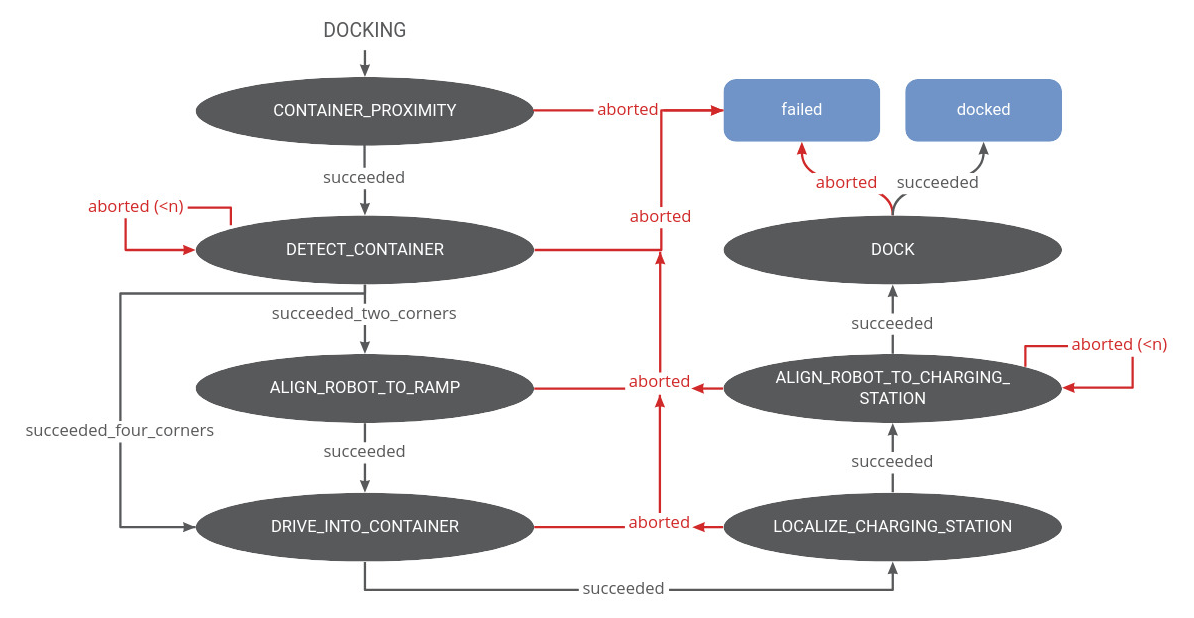
\includegraphics[width=0.8\textwidth]{img/docking_smach.png}
    \caption{\textsc{Docking State Machine}}
    \label{fig:docking_smach}
\end{figure}
\noindent
The first state is \code{CONTAINER_PROXIMITY}, which assumes that the robot has navigated close to the container, e.g., based on GNSS (cf. fig. \ref{fig:container_view}).
Subsequently, if this is the case, \code{DETECT_CONTAINER} begins based on a laser scan recorded by the robot facing the container. In simple terms, it performs a \textit{Hough transform}
to detect lines in the scan and uses a large number of tailored rules to find a reasonable combination of line segments that could represent the container. Essentially, the whole
approach is centered around the idea that the container is a relatively simple geometric shape that can be detected in a laser scan - a combination of line segments
(cf. fig. \ref{fig:rviz_view}).
\begin{figure}[H]
    \centering
    \begin{subfigure}[b]{0.49\textwidth}
        \centering
        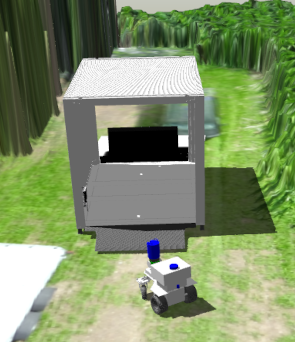
\includegraphics[width=0.55\textwidth]{img/container_view.png}
        \caption{\textsc{Robot Facing the Container}}
        \label{fig:container_view}
    \end{subfigure}
    \hfill
    \begin{subfigure}[b]{0.49\textwidth}
        \centering
        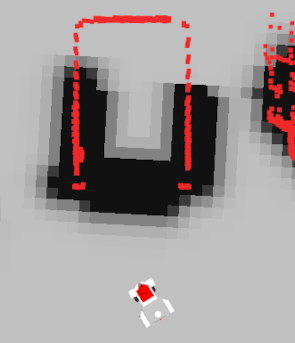
\includegraphics[width=0.55\textwidth]{img/rviz_view.png}
        \caption{\textsc{Container Perception Based on Lidar}}
        \label{fig:rviz_view}
    \end{subfigure}
\caption{\textsc{Container Perception - Geometric Shape}}
\label{fig:container_geometric_shape}
\end{figure}
\noindent
Initially, the input \code{LaserScan} in which the container is to be detected is transformed into the parameter space constructed by spanning the space of possible parameter
combinations, often called \textit{Hough space}. Typically, when using a Hough transform for line detection, the lines are represented in normal parametrization
$\rho = x \cos{\theta} + y \sin{\theta}$, as suggested by Duda et al. \cite{Duda:1972}. Hence, the Hough space is a $2D$ space based on the two parameters $\rho$ and $\theta$. Points
$(x, y)$ on a line in the original Euclidean space intersect in a point, i.e., a $(\rho, \theta)$ combination, in Hough space. The basic idea is to transform each point in the laser
scan into Hough space and count for every parameter combination $(\rho, \theta)$ the number of occurrences. A maximum corresponds to a \textquote{best} match of a line in Euclidean
space. It is therefore reasonable to look for $(\rho, \theta)$ combinations with many hits in Hough space as promising container side candidates.\newline

\noindent
Of course, it is not sufficient to
simply detect lines, because lines occur frequently in the robot's natural environment, not just as part of the container. Nevertheless, the result of this line detection serves as
the basis for the following container detection. It is trivial to calculate the corresponding points that are actually part of the original scan based on the detected lines, so that
the characteristics of the actual line segments that are part of the scan can also be taken into account. Starting with the most prominent line, i.e., the line with the most hits in
Hough space, container detection begins. The initial step is to evaluate whether this baseline candidate could really be a side of the container based on its properties. The first
line segment that matches in this sense, starting with the line with the most hits, followed by the next best lines, is selected. Then, for this line segment, the remaining line
segments that in combination could form the basic shape of the container are considered, in turn ordered decreasingly by their hits in Hough space. The idea is to determine if the
detected line segments meet several criteria that support their plausibility in terms of being a possible container side. For instance, each newly considered line segment must have
an appropriate distance to the previously recognized segments. Appropriate means that the distances do not contradict the dimensions of the container. Moreover, they must be
orthogonal or parallel to all previously detected line segments and their length should not exceed the longest side of the container. However, it is crucial not to be too restrictive,
for example, it must be permissible to undercut the shortest side, due to the fact that the sides may be partially covered. In addition, because of the expected geometric shape of the
container, i.e., a combination of three to four lines, there can be only two lines with approximately the same angle. This fact is used to determine if a newly considered line segment
could still be part of the container candidate. Furthermore, the (infinite) lines must have feasible intersections that match the dimensions of the container. Based on the
intersections of the final set of candidate lines (green lines in fig. \ref{fig:detection_success}) that could represent the container, it can be verified that there must be two segments that exactly satisfy the container width and
two segments that exactly satisfy the container length. At this point, potentially occluded sides are irrelevant as the intersections are based on the angular orientation of the
infinite lines, which is why the resulting dimensions should precisely match the actual known container dimensions. It is of course important to provide a certain tolerance for all
these measurements to ensure practical functionality. There are numerous other details to the container recognition, but the broad ideas of the detection process should be clear.
The result of a successful detection is depicted in fig. \ref{fig:detection_success}, where the four blue boxes represent the corners of the detected container shape, the yellow
box indicates the center, and the cyan arrow marks the target pose of the robot inside the container.
\begin{figure}[H]
    \centering
    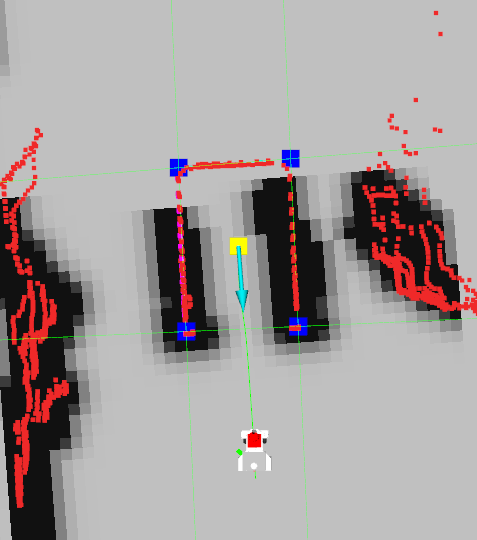
\includegraphics[width=0.34\textwidth]{img/detection_success.png}
    \caption{\textsc{Successfully Detected Container Shape}}
    \label{fig:detection_success}
\end{figure}
\noindent
As a result of a successful execution of \code{DETECT_CONTAINER}, either two or four corners are detected and passed to the next state. If only two corners, i.e., the entry, are
detected, \code{ALIGN_ROBOT_TO_RAMP} follows. If, on the other hand, four corners are detected (cf. fig. \ref{fig:detection_success}), this state is skipped and \code{DRIVE_INTO_CONTAINER} follows, since the entire
container has already been detected. In \code{ALIGN_ROBOT_TO_RAMP}, the robot is aligned in front of the container based on the detected entry. The target pose is passed as the
output of \code{DETECT_CONTAINER} and the robot navigates there. Subsequently, \code{DRIVE_INTO_CONTAINER} follows. If the transition comes from \code{DETECT_CONTAINER}, i.e., if
\code{ALIGN_ROBOT_TO_RAMP} is skipped, all four corners are already detected in the previous state, which are now utilized. If, on the other hand, it follows the state
\code{ALIGN_ROBOT_TO_RAMP}, there is no input and the robot should detect the entire container from the improved position. In both cases, based on the four detected corners,
a pose is computed in the center, facing the entrance, and the robot is navigated there (cf. cyan arrow in fig. \ref{fig:detection_success}). Thereafter, \code{LOCALIZE_CHARGING_STATION} starts using the input corners detected in the
previous state as input. As the mounting position of the charging station within the container is known, the target position for the alignment in front of it can be computed
relative to the detected container shape. Afterwards, the robot is moved there in \code{ALIGN_ROBOT_TO_CHARGING_STATION} and the whole execution of the state machine ends in
\code{DOCK}. Analogously, the undocking state machine ensures that the robot leaves the container after a successful charging procedure to continue its mission.
Finally, it is advisable to clear the costmaps, as parts of the floor are often misconceived as obstacles during ramp traversal.\newline
This (un-)docking solution can be used for both planned charge stops as well as unexpected but necessary stops indicated by monitoring processes such as the one described in section
\ref{sec:battery_monitoring}. Concluding, it is a simple matter to configure whether the simulation should use the docking solution in combination with the container model or only the simplified
charging patch. Similar to Hawes et al. \cite{Hawes:2017} and Pinillos et al. \cite{Pinillos:2016}, one could exploit the fact that the
robot keeps returning to the charging station by resetting the position to the location inside the container aligned in front of the charging station to avoid cumulative localization
errors, thus using the container as a landmark.
